\documentclass[12pt]{article}

\title{Research paper}
\author{Wessel Stoop, s0808709}

\usepackage{covington}
\usepackage{graphicx}
\usepackage{natbib}

\renewcommand{\familydefault}{\sfdefault}

\begin{document}
\maketitle

\section{Introduction}

When one of Starfleet's vessels meets an alien ship in areas where no man has gone before, they can (almost) always communicate with these aliens (almost) instantly; they speak to them in English, and these aliens answer in English. This is possible because, according to the Star Trek lore, the protagonists make use of a so-called Universal Translator. This Universal Translator can (1) recognize speech in every language, (2) translate what it has 'heard' to any other language, (3) make its results audible with speech synthesis and (4) learn itself new languages when needed. Unfortunately, like many technologies in Star Trek, this is far from reality: there is lots of active research at the first three tasks in particular (and even some of the fourth, see \citet{biemann11}), but no software currently in existence can do this as perfect as the Universal Translator. \\\indent
In this paper, I will give a detailed overview of the research project Colibri, which basically is an attempt to improve the technology needed for the second task: automatically translating text from one language to another. More specifically, the project investigates the effects of various translation units; for example, whether making use of constructions with one or more gaps or context improves translation quality. Importantly, the translation is not done on the basis of explicit 'human' knowledge about language and grammar ('linguistic theory'), but are distilled from large amounts of text ('text corpora'). The Colibri project is carried out by Maarten van Gompel and supervised by Antal van den Bosch.
\\\indent
In section 2, I will give a short overview of what has been achieved in machine translation, and in section 3 the current project will be described. This order was chosen to show that Colibri builds on previous research directly. I give more information on the methodology in section 4, and describe the current and future station section 5. Section 6 elaborates on Colibri's relevance, both for science and society, and section 7 describes some strengths and weaknesses of the project. The paper is concluded in section 8.







\section{Theoretical background / framework}

In this section I will try to give a short overview of the various approaches in machine translation, with special attention to the example-based approach, as that is the approach used in this project. This section is mainly based on \citet{jm09} and \citet{vangompel09}.

\subsection{The rule-based approach}

The rule-based approach, also known as Classical Machine Translation, is best characterized by the use of human created rules. That is, authors of translation algorithms tried to include their knowledge about the languages and translation. The rule-based approach can be subdivided into four subapproaches, summarized in the Vauquois triangle: \\

\begin{figure}[htb]
\centering
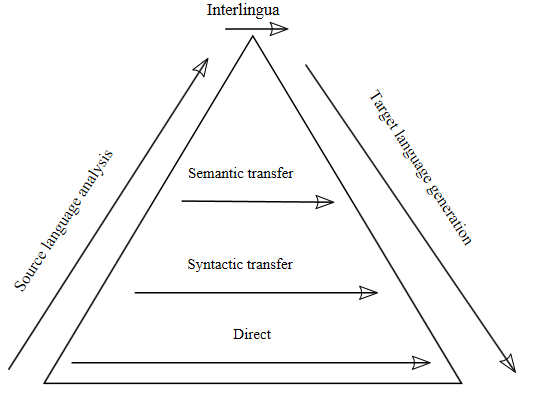
\includegraphics[width=0.8\textwidth]{vauquois.png}
\caption{The Vauquois triangle}
\label{fig:vauquois}
\end{figure}

The horizontal arrows represent the approaches. I will go through them from bottom to top:

\begin{itemize}
\item \emph{The direct approach} does very little source language analysis, and could thus be viewed as the automated version of looking up every word in the source language in a dictionary and replacing it with the corresponding word in the target language. This often does not yield very good results: if I for example would have translated this paper from my mother tongue Dutch to English word for word, 'would we now not real a good result have'. It should be noted, however, that the direct approach mostly is more complicated than this; for example, in some cases morphological analysis is needed before it can be looked up in a dictionary, and more morphological analysis is needed for the translation word to fit in the sentence. Word reordering rules can also be included.
\item \emph{The syntactic approach} tries to discover the syntactic structure of the source sentence before it starts translating, using a parser. This structure is then translated to the target language, and filled with translated words.
\item \emph{The semantic approach} goes even one step further and also tries to grasp the meaning of a sentence, roughly. A sentence like \emph{Mummy kisses daddy} for example entails that mummy is the agent, and daddy the patient of the sentence. After having identified these semantic roles, the algorithm would then look how this meaning is expressed in the target language, find the appropriate syntactic structure for that, and fill it with the translated words.
\item \emph{The interlingua approach}. All of the approaches so far have in common that they require a separate rule set for each language pair; no or very few rules included for translations from English to German can also be used for translations from English to French. This means that for every time a new language is added to the system, the amount of rules that have to be added grows exponentially. The Interlingua approach is an attempt to solve this problem, by pairing up every language with a formal representation of meaning, the Interlingua. This means a translation from English to German would entail a translation from English to the Interlingua (using the ruleset English $\rightarrow$ Interlingua) and then a translation from the Interlingua to German (using the ruleset Interlingua $\rightarrow$ German). When translating from English to French, the same two steps would be taken, and the same ruleset English $\rightarrow$ Interlingua can be used.
\end{itemize}

I should add that translation systems focussing on one approach are rare. As \citet{jm09} put it: 'Real systems tend to involve combinations of elements from these three architectures; thus, each is best thought of as a point in an algorithmic design space rather than as an actual algorithm.' The Systran system \citep{hs92,senellartea01}, for example combines the first three approaches.\\\indent
An advantage of the rule-based approach is that one has a lot of control over the output. In theory, if something has gone wrong, all one has to do is find out which rule or dictionary item caused the problem and improve it. In practice, however, it is almost impossible to have a dictionary and rule system good enough for more complicated sentences, and things like rule interactions and ambiguity make everything even more complicated. The next two approaches therefore replace hand-crafted rules with automatically generated ones.

\subsection{The statistical approach}

Unlike the rule-based approach, the statistical approach creates its own 'knowledge', using bilingual text corpora. This knowledge is probabilistic: instead of using fixed rules, statistical machine translation systems only know how likely a particular translation is on the basis of the data it has seen before. On the basis of these data, various translation hypotheses generated, from which the best one is chosen according to various statistical measures. I will explain these stages in more detail:

\begin{itemize}
\item \emph{Corpus alignment.} Only having a bilingual corpus is not enough: for such a corpus to be useful one also needs to know which parts of the text in language A correspond to which parts of the text in language B. This goes for both the sentence level (which sentence in language A corresponds to which sentence in language B), and the word level (which word in sentence X in language A corresponds to which word in sentence X in language B). Aligning words and sentences is complicated by the fact that sometimes language A uses more or less sentences/words than language B to express the same concept. After aligning words, it is possible to extract aligned phrases on the basis of word-alignment information. \citet{koehn03} show this provides better results than word-based translation.

\item \emph{Hypothesis generation.} We now have some sort of automatically generated dictionary for each word or phrase in language A, we know which word or phrase in language B is often used for it, and with what probability. In phrase-based machine translation, this dictionary is called the \emph{phrase translation table}. On the basis of this dictionary or phrase translation table, we can generate various possible translations. \\\indent

\item \emph{Hypothesis evaluation.} Which one of these possible translations is the best one is determined on the basis of two measures: faithfulness and fluency (which could also be called grammaticality). These measures often are in conflict: a solution to get an optimally fluent translation would be to always return the same well-formed sentence, but that would not be faithful to the source sentence at all, while a very faithful translation, for example translating a sentence word by word, is usually not considered very fluent. Faithfulness and fluency are measured by the translation model and the language model respectively:

\begin{itemize}
\item \emph{The translation model.} The translation model returns a probability of the source sentence given the target sentence; it thus looks back whether what has been created fits the original. This probability is calculated on the basis of statistical word alignment algorithms like the IBM models \citep{brown93}.

\item \emph{The language model.} The language model predicts to what extent the generated sentence is expected for the target language; in other words, is this sentence a well-formed sentence or not? Because the unlimited number of ways words can be combined into sentences, it is unlikely the sentence under investigation will actually be found in a corpus, so the language model tries to do this prediction on the basis of how often smaller parts of the sentence (n-grams) occur in a corpus in sequence.

\end{itemize}

\end{itemize}

The algorithm that performs the last two steps, hypothesis generation and evaluation, is called a \emph{decoder}. I should add that, in practice, not all possible hypotheses will be generated and evaluated, because that would take too much time and memory. Instead, the decoder's task could be viewed as search problem: we have an enormous pile of possible hypotheses of which one is this best, and we want to find that one hypothesis as quickly and efficiently as possible. To achieve this, only a small set of hypotheses is generated and evaluated immediately. New hypotheses are only generated on the basis of the outcomes, elimating search directions which are very unlikely to produce good results. In other words, in actual translation systems hypothesis generation and evaluation are mostly intertwined. 

\subsection{The example-based approach}

For my overview of the example-based approach, I will focus on the memory-based version of the example-based approach in particular, because that is the version the Colibri project uses. Other versions of example-based machine translation might vary slightly. \\\indent
The memory-based approach is in many ways similar to the statistical approach - it could even easily be argued to be a part or an extension of it. For example, the memory based approach also generates translations on the basis of large bilingual corpora, and also works with a decoder to mold the various translation pieces found into a sentence. The main difference, however, is that it takes the context of the source language into account; the idea is that the system will find another translation for \emph{left} in the sentence \emph{The toilets are at your left hand} than for \emph{left} in the sentence \emph{Elvis has left the building} simply because they occur in different contexts. \\\indent
In the memory-based approach, this context-sensitivy is achieved with the help of machine learning: by showing a so-called classifier lots of examples of something, and telling it to which class it belongs, the classifier is able to predict the class of new examples. For example, we can give a classifier the external characteristics of 10.000 humans (length, type of cloths, length of hair, etc.), and also tell it whether these humans are male or female. If we then ask for the sex of a relatively short human, wearing a dress, with long hair, the classifier will probably be able to tell us this is a woman, because most of the examples with similar features also were women. It thus is frequency that plays a central role here.\\\indent
While this example only has two classes, it is in principle possible to use a very large number of classes. This is exactly what the memory-based approach to machine translation does: on the basis of a particular word and its context (for example, its direct neighbours), a classifier in machine translation returns as a class the most likely translation. Thus, instead of on human characteristics the classifiers are trained on words and their context from the source language, and instead of sex it uses n-grams from the target language as classes. \\\indent
There are two types of classification methods: \emph{eager learning} and \emph{lazy learning}. Whereas eager learning algorithms try to create a small, abstract, general model, filtering out infrequent cases, lazy learning algorithms take into account everything they encounter. According to \citet{dvdb05}, for natural language processing the lazy learning approach works best, because infrequent cases are an important part of the knowledge needed. \\\indent
Like I did with statistical machine translation, I will now give an overview of the memory-based machine translation process, adapted from \citet{vdbb09}. For this example, I will describe a translator that uses trigrams, but all kinds of n-grams could be used here, even n-grams of variable length. In fact, \citet{vangompel09}, \citet{vangompelea09} and \citet{vangompel11} showed that better results can be achieved using phrases of variable length; investigating the nature of multi-word units in translation therefore is one of the main goals of the Colibri project.

\begin{itemize}
\item \emph{Training.} Training is done only once and \emph{before} actual translation, and could therefore be seen as 'preparing' the translation software for its task. It consists of (1) aligning the bilingual corpus, using the word alignment algorithms described in the previous sections, (2) decomposing the complete corpus into trigrams, and (3) creating a translation model on the basis of this. The trigrams of the source language constitute the examples, the trigrams of the target language are the classes.

\item \emph{Local classification.} Classification means (1) decomposing the source text into trigrams and (2) classifying each trigram, based on the translation model created in the training phase. The output are the classes, i.e. the trigrams, the classifiers associates with each source trigram.

\item \emph{Global search.} In the global phase we try to merge the trigrams into one text. The part of the translation software responsible for this is called the \emph{decoder}. There might be a lot of overlap in the resulting trigrams (for example, when the trigrams would be '\emph{\_ I love}', '\emph{I love you}' and '\emph{love you \_}'), making the decoder's task relatively easy. Such overlap might even give hints for the word order of the target language. In many cases, unfortunately, such overlap does not exist or is even misleading. As with statistical translation, here too we can pick the best translation hypothesis by using a language model and a translation model. 

\end{itemize}

Please note again the similarities with the statistical approach: like in the \emph{hypothesis generation} phase, (parts of) hypotheses are generated during \emph{local classification}, and like the \emph{hypothesis evaluation phase}, hypotheses are evaluated during \emph{global search}.





\section{Project description} \label{Description}

Colibri is an attempt to improve the quality of machine translation. This is done by building a translation system using state-of-the-art techniques, then implementing new concepts, and investigating whether they improve translation quality or not. Two concepts investigated so far are the use of constructions instead of phrases as translation units, and the use of context while translating these units. In section \ref{constructions}, I will describe what constructions are and why they might improve translation, in section \ref{builder} I describe the actual software that uses these constructions \emph{and} their context.

\subsection{The building blocks: constructions} \label{constructions}

Colibri, 'Constructions as Linguistics Bridges', investigates constructions, as its name suggests. A construction can be any group of consecutive words that in some way forms an entity, in any natural language. An example is 'on the basis of' in the following sentence:

\begin{examples}
\item On the basis of these ideas, software can be developed.
\end{examples}

Importantly, constructions can also have one or more gaps (so-called 'skipgrams'). 'From \_\_ point of view' in the following example, is a construction with one such gap. 

\begin{examples}
\item I understand things better when I look at them from his point of view.
\end{examples}

The gap here is filled with 'his', but the construction 'from \_\_ point of view' can also be filled with many other words ('my', 'the', 'another', 'Obama's', etc.). This shows the appeal of skipgrams over n-grams for machine translation: whereas n-grams would only have been able to capture the construction 'point of view', because the word directly before 'point of view' is variable, skipgrams are also able to recognize that the word 'for' is part of the construction. Frequent examples of the skipgrams (I expect the variant with 'my' to be very frequent, for instance) of course \emph{could} be recognized by the n-gram approach.\\\indent
Of course, not every possible group of consecutive words is a construction; what makes some groups special? The exact nature of linguistic constructions has been the subject of many linguistic publications and even an entire group of linguistic frameworks (construction grammar, see \citet{goldberg95} for a well-known example). For this project, however, it suffices to say that constructions emerge because some combinations of words are more frequent than others. As we have seen in the previous section, taking into account frequency in the training material is how classifiers are able to do their job.

\subsection{The builder: machine translation} \label{builder}
Besides an attempt to discover more about the possibilities for machine translation technology, Colibri is also an attempt to actually develop this technology. A project overview therefore cannot be complete without an overview of the software's functionality. Colibri's functionality can be split in four parts: (1) identifying and extracting constructions in a language, (2) identifying aligned constructions between language-pairs, (3) memory-based classification and (4) reassembling constructions into a coherent target sentence. I will discuss the four parts in more detail consecutively:

\subsubsection{Identifying and extracting constructions in a language}
When using large corpora, the process of discovering simple n-grams might already take quite a lot of time and memory; adding variability in length and one or multiple gaps to the n-grams makes the process even more - in fact, many times more - complex. To reduce the processing load and resource consumption, two techniques are used:

\begin{itemize}
\item Optimization of how the various the n-grams and skipgrams are saved in memory. By reserving the labels that do not take a lot of memory for the most frequent grams, a lot of memory can be saved.
\item For trigrams and larger n-grams, taking into account the frequencies of the parts. If these parts do not exist or are very infrequent, there is no use in looking for the whole - if even the parts do not exist, the whole will not exist for sure and does not need to be investigated any further.
\end{itemize}

\subsubsection{Identifying aligned constructions between language-pairs}
Once the constructions in both parts of a bilingual corpus are identified, these constructions need to be linked. Colibri aligns constructions by aligning the individual words first and constructions later, and uses a separate algorithm to align skipgrams.\\\indent
It should be noted that this approach is the result of various investigations. For example, instead of the classical approach of aligning constructions by aligning the individual words first, as described by \citep{koehn03}, it was attempted to try to align the constructions directly. To achieve this, one can for example simply measure how often the constructions found in both languages occur together (that is, in both the source and the target language). Because at this stage the decoder was not yet ready (see subsection 4), the decoder from translation system MOSES \citep{koehnea07} was used to evaluate the results. These results showed that the approach using constructions directly for alignment could not provide results as good as the approach mediated through word alignments; therefore, it was decided to go back to the classical method. It should be noted that, because the MOSES decoder was used, the influence of skipgrams on alignment could not be measured. However, because they increase complexity, they are not expected to improve the alignments.\\\indent
When support for skipgrams was added to the implementation of the classical approach, it turned out that including skipgrams in the alignment process had negative effects on the results. To fix this, an algorithm specialized for aligning skipgrams was developed, which indeed was able to find good translations. 

\subsubsection{Memory-based classification}
As may have become clear from the previous sections, the Colibri project investigates the use of machine learning techniques to get from the source language construction to the target language constructions. Three approaches have been implemented:

\begin{itemize}
\item Monolithic classifier. All phrases go through one general classifier. This classifier thus has a very large number of classes to pick from.
\item N-array classifiers. There is a separate classifier for each phrase length (n); the length of the source language construction thus decides which classifier is used.
\item Construction experts. Each construction or phrase has its own classifier, which means that instead of one larger classifier, there are a lot of smaller classifier making a simpler decision. This is inspired by the effectivity of this approach in word sense ambiguation \citep{vangompel10}.
\end{itemize}

\subsubsection{Reassembling constructions into a coherent target sentence}
A decoder was developed from scratch, following state-of-the-art techniques as described by \citet{koehn03}. Support for skipgrams and machine learning, of course not available in standard decoders, was added.




\section{Methodology}

Because of Colibri's practical nature, its methodology forms the core of the project and has been explained in detail in the previous sections, making this section largely superfluous. The only thing I would like to give some attention is that Colibri's time planning is similar to that of other research projects:

\begin{enumerate}
\item reading the previous literature
\item building a theoretical model
\item testing the model, for example with experiments
\item refining the model on the basis of the results
\end{enumerate}

However, what is actually done during these stages is radically different from many other fields of science. For example, whereas stage 2 in many research projects will result in a paragraph of text, a table, a flowchart, a formula, or something similar, Colibri's stage 2 actually results in a fully functional translation system. And whereas stage 3 in many fields of science entails designing some kind of experiment that will hopefully provide evidence for the model developed during stage 2 (and then finding people to participate in that experiment), Colibri's stage 3 consists of writing a script to evaluate the results of the translation system, using various evaluation measures.




\section{Current status and future research}

At the moment, the functional machine translation system described in section \ref{builder} is mostly finished. It is mainly inspired upon the open source translation system MOSES, and indeed manages to produce similar results. However, as was explained in section \ref{Description}, Colibri is an attempt to improve the quality of machine translation by adding skipgrams and memory-based learning. Unfortunately it has turned out that both do not add much to the translation quality: all three memory-based learning approaches (construction experts, N-array classifiers and a monolithic classifier) only improve the results a little bit, and the skipgrams are mostly ignored by the decoder. Apparently, translation hypotheses without skipgrams are more likely to be good translations in most of the cases. \\\indent
This means Colibri's goal, improving translation quality, has not yet been achieved. It is possible that larger improvements in translation quality \emph{can} be achieved by changing things like corpora or even languages used, but if this is not the case, new possibilities for improvements have to be investigated. One such possibility is to include a system that finds the correct translations of words on the basis of particular keywords in a sentences. This system should for example be able to translate the English \emph{bank} into Dutch \emph{oever} ('river bank') when the words like \emph{boat} are mentioned, but into \emph{bank} (financial institution) when \emph{money} is mentioned.




\section{Relevance}

\subsection{For science}

Because Colibri's goals are not reached at the moment and there currently is no certainty about whether this will happen, Colibri's scientific relevance for now is relatively small; as described in the previous section, the already existing open source machine translation system MOSES has similar results. I should add, however, that the current state the project is in seems to be a fertile ground for breakthroughs in the future. 

\subsection{For society} \label{soc}

Assuming such a breakthrough will indeed come, the relevance for society is a big one: by improving the quality of machine translation, one basically improves (1) to what extent someone can get information from a document written in a human language he or she does not master, and (2) to what extent people without a common language can communicate. As for the first point, a lot of the roughly 7000 languages in the world also have a written form. This means that, unless you know all of these languages, part of all information available can only be reached by translation. This can of course be done a translator, but that is a time-consuming and labour-intensive job, which forces us to concentrate on translating only the more important documents to the more important languages. With good machine translation, we can easily make available \emph{all} information available to everyone. The second point is perhaps even more important: if for two people there is not a language they both speak, they have very few ways to communicate. In practice this means whole communities of people are excluded from the rest of the world, simply because they do not know the languages of the rest of the world. In highly educated societies this is of course less of a problem, as people can easily learn a new language as long as they are willing to do some effort, but foreign language education is not available in large parts of the world. If it manages to get good enough, machine translation might save the day here: by building 'linguistic bridges' between the world's communities, it creates the possibility for everyone on the globe to communicate with everyone on the globe. This means one is no longer limited to the community he or she was born, which may increase one's chances for a happy and succesful life significantly.






\section{Strengths and weaknesses}

In this section, I will try to give an overview of the project's strong and weak points. Some points concern this particular research project, other concern the memory based approach, and others zoom out even further and concern machine translation in general.

\subsection{Strenghts}

Besides the general strength described in section \ref{soc}, Colibri has (at least) two more:

\subsubsection{The theory is tested immediately and completely}

An idea is very different from something that is really useful or true. Many fields of science get stuck somewhere in this transition. In some fields scholars only write down their ideas in human language, not fully formulating how the idea should work, and thus never discovering there might be flaws in the idea somewhere. In other fields scholars can make the idea formal, but have no way to test the ideas in any other way than trusting on intuitions. In again other fields one can test it, for example by means of experiments, but it remains unclear how the results should be interpreted and to what extent they generalize to the whole population. All this is not a problem for the Colibri project. Claims are made (for example 'skipgrams improve machine translation'), formalized ('this is how they should work within in a machine translation system'), but also implemented and tested in a fully functional machine learning system. In other words, except maybe for the evaluation measures, there is little reason to doubt the results of this project, because of its highly emperical nature. 

\subsubsection{The example-based approach makes the system easily extensible to other languages}

When describing the rule-based approaches to machine translation, I pointed out that for most approaches one needs a specific ruleset for each language pair. The Interlingua approach is an attempt to solve this problem by adding a language in between, so that only a ruleset for every language $\rightarrow$ Interlingua and Interlingua $\rightarrow$ language pair is needed. Statistical and memory-based approaches solve this problem in an even more elegant way: the only things needed are computational power, time, and a lot of data. As digital translated texts are available in large quantities for the more important languages of the world, adding more languages to Colibri should be relatively easy. But even less important languages can be added easily, as long as there is enough data to train the translation model (but see the first two weaknesses). Obviously, the opposite is true for the rule-based approach.

\subsection{Weaknesses}

\subsubsection{Memory based learning depends on quantity and quality of the data}

Statistical and Memory-based machine translation takes the rule-creating process out of the hands of the authors. This can be a good thing, because it means translation systems can be made without any knowledge of the source or the target language, but it also means the authors loses control over what the system produces. That is, if the system makes errors, solving this problem is not as simple as changing how the system works. \\\indent
Instead, the task of the creator now is to provide enough bilingual texts for training - preferably as much as possible - as this improves the change of finding a matching n-gram. These data are simply not available for all languages in the world. And not only should there be enough bilingual texts, they should also be of high quality. One incorrect translation, if not found anywhere else in the corpus, can already end up in the translation results. For example, when translating \emph{Will Justin Bieber ever hit puberty} from English to Vietnamese with Google Translate, which is also based on bilingual corpora, the result is \emph{Justin Bieber se bao gio den tuoi day thi}, which means as much as 'Justin Bieber will never hit puberty'.

\subsubsection{It is unclear how well the memory-based approach works for languages with a more free word order}

Memory-based learning generates a translation on the basis of source-context. This works well for languages in which word order is largely fixed, like English: for these languages, if you change the position of a particular word in the sentence (and thus the context), you also change the meaning of that sentence. There are languages, however, with relatively free word order; Hungarian, Russian and Finnish, to name a few. In these languages, changing the position and thus the context of a particular word or phrase does not (really) change the meaning of the sentence. In other words, in these languages the main source of the knowledge of memory-based learning is not fully available, which may very well mean that memory-based translation may not be useful for these languages. On the other hand, in many languages with free word order there is something like a canonical word order (so, although the order is free, it is not random), and almost all languages with free word order use case instead. Case could be really useful to memory-based learning, because having a word in a particular case in the context might be a very good clue which possible translation is the best. To what extent free word order is a problem or case is helpful is completely unclear.
\\\indent

\subsubsection{Machine translation is not good for the common view on translation}

Machine translation is far from perfect. Colibri of course is an interesting attempt to bring the technology closer to the 'perfect' end of the scale, but it will almost certainly not result in an application which is able to replace human translators. However, when non-perfect software like this is made available to the public, ignorant users might treat it as if it was perfect software, thereby turning off their own intelligence, as it were. A similar criticism can be heard in the field of spell checkers: the invention of automated  spell checkers would have caused a general trend in relying on the technology too much, and regarding work as finished without even proofreading it. \citet{galletta05} for example show that people deliver texts with more false-positive and false-negative errors in it when a spell checker was present, and that this even holds for people with good verbal skills. \\\indent
Although giving a detailed analysis of this viewpoint is beyond the scope of this paper, I would like to point out that something similar already seems to be happening for machine translation: since the release of Google Translate, various examples of websites, street signs, restaurant menus and other texts incorrectly translated by the service can be found on the internet. The authors of the text, apparently not skilled in the target language, have relied on machine translation only and did not check the quality translation in any other way.\\\indent
And to make the problem even more complicated, there probably is no such thing as a 'correct' translation, in contrast to what the previous paragraphs may have suggested. That is, if you ask \emph{n} translators to translate a long text from language A to language B, \emph{n} different translations will be produced. Translation is a problem for which no clearly defined answer exists. Instead, what one considers a good translation is largely a matter of taste, beliefs, cultural preference, etc., making translation much closer to an art. Viewing translation as something a computer can do might be a huge underestimation of the task, and giving the ignorant user this impression could be argued to be very misleading.







\section{Conclusion}
In this paper, I hope to have given a good impression of the research project Colibri. Various approaches to machine translation were described, among which memory-based learning, the approach Colibri uses. After that Colibri itself was discussed in more detail, from various viewpoints. We saw how the project is organized, and that skipgrams and context-sensitivity were investigated as possible innovations to machine translation, but also how building a practical application has importantant advantages for doing research, and what improving machine translation might mean for society.

\begin{thebibliography}{99}

\bibitem[Biemann, 2011]{biemann11}
Biemann, C. (2011). \emph{Structure discovery in natural language.} New York / Dordrecht: Springer.

\bibitem[Van den Bosch \& Berck, 2009]{vdbb09}
Van den Bosch, A., \& P. Berck (2009). Memory-based machine translation and language modeling. \emph{The Prague Bulletin of Mathematical Linguistics}, 91, 17\-26.

\bibitem[Brown et al., 1993]{brown93}
Brown, P. F., V. J. D. Pietra, S. A. D. Pietra \& R. L. Mercer (1993). The mathematics of statistical machine translation: parameter estimation. \emph{Computational Linguistics}, 19(2), 263–311.

\bibitem[Daelemans \& van den Bosch, 2005]{dvdb05}
Daelemans, W. \& A. van den Bosch (2005). \emph{Memory-based language processing}. Cambridge, UK: Cambridge University Press.

\bibitem[Dempster et al., 1997]{dempster77}
Dempster, A. P., N. M. Laird, \& D. B. Rubin (1977). Maximum likelihood from incomplete data via the em algorithm. \emph{Journal of the Royal Statistical Society}. Series B (Methodological), 39(1), 1–38.

\bibitem[Galletta et al., 2005]{galletta05}
Galletta, D. F., A. Durcikova, A. Everard \& B. M. Jones. Does spelling checker software need warning label? \emph{Communications of the ACM}, 48(7), 82-86.

\bibitem[Goldberg, 1995]{goldberg95}
Goldberg, A (1995). \emph{Constructions: A Construction Grammar Approach to Argument Structure.} Chicago: University of Chicago Press.

\bibitem[Van Gompel, 2009]{vangompel09}
Van Gompel, M. \emph{Phrase-based memory-based machine translation.} Unpublished
master's thesis, Tilburg University.

\bibitem[Van Gompel et al., 2009]{vangompelea09}
Van Gompel, M., A. Van den Bosch, \& P. Berck (2009). Extending memory-based machine translation to phrases. In M. Forcada \& A. Way (Eds.), \emph{Proceedings of the third workshop on example-based machine translation} (pp. 79\-86). Dublin, Ireland.

\bibitem[Van Gompel, 2010]{vangompel10}
Van Gompel, M. (2010). Uvt-wsd1: A cross-lingual word sense disambiguation system. In \emph{Semeval '10: Proceedings of the 5th international workshop on semantic evaluation} (pp. 238-241). Morristown, NJ, USA: Association for Computational Linguistics.

\bibitem[Van Gompel et al., 2011]{vangompel11}
Van Gompel, M., A. Van den Bosch, \& P. Berck (2011). Extending memory-based
machine translation to phrases. In T. Markus, P. Monachesi, \& E. Westerhout (Eds.), \emph{Computational linguistics in the netherlands 2010: Selected papers from the twentieth clin meeting} (pp. 45-58). Utrecht, the Netherlands: LOT.

\bibitem[Van Gompel, 2012]{vangompel12}
Van Gompel, M. (2012). \emph{Colibri documentation}. Available online at http://proycon.github.com/colibri/doc/.

\bibitem[Hutchins \& Somers, 1992]{hs92}
Hutchins, W. J. \& H. L. Somers (1992). \emph{An introduction to Machine Translation.} Academic Press.

\bibitem[Jurafsky \& Martin, 2009]{jm09}
Jurafsky, D. \& J. H. Martin (2000). \emph{Speech and language processing: an introduction to natural language processing, computational linguistics, and speech recognition.} Second edition. New Jersey: Pearson Education.

\bibitem[Koehn et al, 2003]{koehn03}
Koehn, P., F.-J. Och, \& D. Marcu (2003). Statistical phrase-based translation. In \emph{Proceedings of hlt-naacl 2003} (pp. 48-54). Edmonton, Canada.

\bibitem[Koehn et al, 2007]{koehnea07}
Koehn, P., H. Hoang, A. Birch, C. Callison-Burch, M. Federico, N. Bertoldi, et al. (2007). Moses: Open source toolkit for statistical machine translation. In \emph{ACL. The Association for Computer Linguistics.}

\bibitem[Senellart et al., 2001]{senellartea01}
Senellart, J., P. Dienes \& T. Varadi (2001). New generation SYSTRAN translation system. In emph{MT Summit 8}.

\bibitem[Stroppa et al., 2007]{stroppa07}
Stroppa, N., A. Van den Bosch, \& A. Way, (2007). Exploiting source similarity for SMT using context-informed features. In A. Way \& B. Gawronska (Eds.), \emph{Proceedings of the 11th international conference on theoretical issues in machine translation (tmi 2007)} (pp. 231\-240). Skövde, Sweden.

\end{thebibliography}

\end{document}
